% questions.tex —— 2020 年·新高考Ⅰ卷（山东） · 题目内容片段（无答案）
% 由 tools/generate_projects.py 依来源总账自 2020/2020_数学真题_新高考1_试题.md 生成，勿手改（改源 MD 后重跑）


\begin{gknotice}
\textbf{来源说明}：本题面依据固定源 PDF 的两页 A3 题面逐题转录，原卷印刷页码为 1133、1134。第 1133 面为单选题 1—8、多选题 9—12、填空题 13—16 与解答题 17、18；第 1134 面为解答题 19—22。原页四处节头依次为「一、单选题」「二、多选题」「三、填空题」「四、解答题」，题号与索引一致；所有数值、分式、根号与上下标均回原页 300—600 dpi 核对。

\textbf{解析归属}：固定源不附答案或解析；配套答案与解析均由本库按本题面独立复算（等级 D，非官方）。

\textbf{图形说明}：第 10 题的正弦型函数图象、第 15 题的零件截面、第 20 题的四棱锥，均由项目内 TikZ 矢量源按原页几何重绘；第 4 题原页为日晷实景照片（纯情境示意、无可读数据），按本库「实景照片不重绘、不入图」的既定规则不入图，题干信息完整保留；其余各题原页无图。

\textbf{评分说明}：原页未印多选题的给分说明。按新高考Ⅰ卷通用规则，多选题全部选对得 5 分，部分选对得 3 分，有选错得 0 分；此条非原页文字，仅作使用提示。
\end{gknotice}

\gkpart{一、单选题}

\begin{question}
\gkti{1}设集合 $A=\{x\mid 1\leqslant x\leqslant 3\}$，$B=\{x\mid 2<x<4\}$，则 $A\cup B=$\mbox{（　　）}

（A）$\{x\mid 2<x\leqslant 3\}$；（B）$\{x\mid 2\leqslant x\leqslant 3\}$；（C）$\{x\mid 1\leqslant x<4\}$；（D）$\{x\mid 1<x<4\}$。

\end{question}
\begin{question}
\gkti{2}$\dfrac{2-\mathrm i}{1+2\mathrm i}=$\mbox{（　　）}

（A）$1$；（B）$-1$；（C）$\mathrm i$；（D）$-\mathrm i$。

\end{question}
\begin{question}
\gkti{3}$6$ 名同学到甲、乙、丙三个场馆做志愿者，每名同学只去 $1$ 个场馆，甲场馆安排 $1$ 名，乙场馆安排 $2$ 名，丙场馆安排 $3$ 名，则不同的安排方法共有\mbox{（　　）}

（A）$120$ 种；（B）$90$ 种；（C）$60$ 种；（D）$30$ 种。

\end{question}
\begin{question}
\gkti{4}日晷是中国古代用来测定时间的仪器，利用与晷面垂直的晷针投射到晷面的影子来测定时间。把地球看成一个球（球心记为 $O$），地球上一点 $A$ 的纬度是指 $OA$ 与地球赤道所在平面所成角，点 $A$ 处的水平面是指过点 $A$ 且与 $OA$ 垂直的平面。在点 $A$ 处放置一个日晷，若晷面与赤道所在平面平行，点 $A$ 处的纬度为北纬 $40^\circ$，则晷针与点 $A$ 处的水平面所成角为\mbox{（　　）}

[第4题图：原页为日晷实景照片，按本库「实景照片不重绘、不入图」规则不入图，题干信息已完整照录]

（A）$20^\circ$；（B）$40^\circ$；（C）$50^\circ$；（D）$90^\circ$。

\end{question}
\begin{question}
\gkti{5}某中学的学生积极参加体育锻炼，其中有 $96\%$ 的学生喜欢足球或游泳，$60\%$ 的学生喜欢足球，$82\%$ 的学生喜欢游泳，则该中学既喜欢足球又喜欢游泳的学生数占该校学生总数的比例是\mbox{（　　）}

（A）$62\%$；（B）$56\%$；（C）$46\%$；（D）$42\%$。

\end{question}
\begin{question}
\gkti{6}基本再生数 $R_0$ 与世代间隔 $T$ 是新冠肺炎的流行病学基本参数。基本再生数指一个感染者传染的平均人数，世代间隔指相邻两代间传染所需的平均时间。在新冠肺炎疫情初始阶段，可以用指数模型：$I(t)=\mathrm e^{rt}$ 描述累计感染病例数 $I(t)$ 随时间 $t$（单位：天）的变化规律，指数增长率 $r$ 与 $R_0$，$T$ 近似满足 $R_0=1+rT$。有学者基于已有数据估计出 $R_0=3.28$，$T=6$。据此，在新冠肺炎疫情初始阶段，累计感染病例数增加 $1$ 倍需要的时间约为（$\ln2\approx0.69$）\mbox{（　　）}

（A）$1.2$ 天；（B）$1.8$ 天；（C）$2.5$ 天；（D）$3.5$ 天。

\end{question}
\begin{question}
\gkti{7}已知 $P$ 是边长为 $2$ 的正六边形 $ABCDEF$ 内的一点，则 $\overrightarrow{AP}\cdot\overrightarrow{AB}$ 的取值范围是\mbox{（　　）}

（A）$(-2,6)$；（B）$(-6,2)$；（C）$(-2,4)$；（D）$(-4,6)$。

\end{question}
\begin{question}
\gkti{8}若定义在 $\mathbf R$ 的奇函数 $f(x)$ 在 $(-\infty,0)$ 单调递减，且 $f(2)=0$，则满足 $xf(x-1)\geqslant0$ 的 $x$ 的取值范围是\mbox{（　　）}

（A）$[-1,1]\cup[3,+\infty)$；（B）$[-3,-1]\cup[0,1]$；（C）$[-1,0]\cup[1,+\infty)$；（D）$[-1,0]\cup[1,3]$。

\end{question}
\gkpart{二、多选题}

\begin{question}
\gkti{9}已知曲线 $C:mx^2+ny^2=1$\mbox{（　　）}

（A）若 $m>n>0$，则 $C$ 是椭圆，其焦点在 $y$ 轴上；（B）若 $m=n>0$，则 $C$ 是圆，其半径为 $\sqrt n$；

（C）若 $mn<0$，则 $C$ 是双曲线，其渐近线方程为 $y=\pm\sqrt{-\dfrac mn}x$；（D）若 $m=0$，$n>0$，则 $C$ 是两条直线。

\Needspace{0.4\textheight}
\end{question}
\begin{question}
\gkti{10}下图是函数 $y=\sin(\omega x+\varphi)$ 的部分图象，则 $\sin(\omega x+\varphi)=$\mbox{（　　）}
\nopagebreak[4]
\begin{center}% 2020 新高考Ⅰ卷（山东）10：函数 y=sin(ωx+φ) 的部分图象
% 绘制依据：固定源 PDF 原页（300—600 dpi 逐像素核对）。读图锚点：
% 相邻零点 π/6（下降）与 2π/3（上升）间距 π/2 = T/2，故 T=π、ω=2；
% 由下降零点 2·(π/6)+φ=π 得 φ=2π/3，即 y=sin(2x+2π/3)。
% 最大值在 x=−π/12（y 轴稍左，恰与刻度 1 齐平）；y 轴上取值为 sin(2π/3)=√3/2；
% 最小值在 x=5π/12；x=11π/12 处再现波峰后下降。
% 取域 x∈[−π/6, 13π/12]：左端 y=sin(π/3)=√3/2，右端 y=sin(17π/6)=1/2，
% 与原页「左端在半高处起笔、右端过波峰后下降到半高附近收笔」一致。
% y 轴只标刻度 1；x 轴只标 π/6 与 2π/3，分置零点左下 / 右下以避让曲线；O 标原点左下。
\begin{tikzpicture}[xscale=1.9, yscale=1.75, font=\small]
  % ---------- 坐标轴 ----------
  \draw[->] (-0.80,0) -- (3.80,0) node[right] {$x$};
  \draw[->] (0,-1.50) -- (0,1.70) node[above] {$y$};
  % ---------- 曲线 ----------
  \draw[thick, domain=-0.5236:3.4034, samples=240]
    plot (\x, {sin(deg(2*\x+2*pi/3))});
  % ---------- 刻度与标注 ----------
  \draw (-0.05,1) -- (0.05,1);
  \node[above left, inner sep=1pt] at (0,1) {$1$};
  \node[below, inner sep=1pt, xshift=-3pt, yshift=-2pt] at ({pi/6},0) {$\frac{\pi}{6}$};
  \node[below, inner sep=1pt, xshift=4pt, yshift=-2pt] at ({2*pi/3},0) {$\frac{2\pi}{3}$};
  \node[below left, inner sep=2pt] at (0,0) {$O$};
\end{tikzpicture}
\end{center}
\nopagebreak[4]
（A）$\sin\left(x+\dfrac\pi3\right)$；（B）$\sin\left(\dfrac\pi3-2x\right)$；（C）$\cos\left(2x+\dfrac\pi6\right)$；（D）$\cos\left(\dfrac{5\pi}6-2x\right)$。

\end{question}
\begin{question}
\gkti{11}已知 $a>0$，$b>0$，且 $a+b=1$，则\mbox{（　　）}

（A）$a^2+b^2\geqslant\dfrac12$；（B）$2^{a-b}>\dfrac12$；（C）$\log_2a+\log_2b\geqslant-2$；（D）$\sqrt a+\sqrt b\leqslant\sqrt2$。

\end{question}
\begin{question}
\gkti{12}信息熵是信息论中的一个重要概念。设随机变量 $X$ 所有可能的取值为 $1$，$2$，$\cdots$，$n$，且 $P(X=i)=p_i>0$（$i=1,2,\cdots,n$），$\sum\limits_{i=1}^n p_i=1$，定义 $X$ 的信息熵 $H(X)=-\sum\limits_{i=1}^n p_i\log_2p_i$。\mbox{（　　）}

（A）若 $n=1$，则 $H(X)=0$；（B）若 $n=2$，则 $H(X)$ 随着 $p_1$ 的增大而增大；

（C）若 $p_i=\dfrac1n$（$i=1,2,\cdots,n$），则 $H(X)$ 随着 $n$ 的增大而增大；

（D）若 $n=2m$，随机变量 $Y$ 所有可能的取值为 $1$，$2$，$\cdots$，$m$，且 $P(Y=j)=p_j+p_{2m+1-j}$（$j=1,2,\cdots,m$），则 $H(X)\leqslant H(Y)$。

\end{question}
\gkpart{三、填空题}

\begin{question}
\gkti{13}斜率为 $\sqrt3$ 的直线过抛物线 $C:y^2=4x$ 的焦点，且与 $C$ 交于 $A$，$B$ 两点，则 $|AB|=$\gkblank{}。

\end{question}
\begin{question}
\gkti{14}将数列 $\{2n-1\}$ 与 $\{3n-2\}$ 的公共项从小到大排列得到数列 $\{a_n\}$，则 $\{a_n\}$ 的前 $n$ 项和为\gkblank{}。

\Needspace{0.4\textheight}
\end{question}
\begin{question}
\gkti{15}某中学开展劳动实习，学生加工制作零件，零件的截面如图所示。$O$ 为圆孔及轮廓圆弧 $AB$ 所在圆的圆心，$A$ 是圆弧 $AB$ 与直线 $AG$ 的切点，$B$ 是圆弧 $AB$ 与直线 $BC$ 的切点，四边形 $DEFG$ 为矩形，$BC\perp DG$，垂足为 $C$，$\tan\angle ODC=\dfrac35$，$BH\parallel DG$，$EF=12\ \mathrm{cm}$，$DE=2\ \mathrm{cm}$，$A$ 到直线 $DE$ 和 $EF$ 的距离均为 $7\ \mathrm{cm}$，圆孔半径为 $1\ \mathrm{cm}$，则图中阴影部分的面积为\gkblank{}$\mathrm{cm}^2$。
\nopagebreak[4]
\begin{center}% 2020 新高考Ⅰ卷（山东）15：某零件的截面（1 单位 = 1 cm，整图 scale=0.75）
% 绘制依据：固定源 PDF 原页逐像素核对。矩形 DEFG：D(0,2)、E(0,0)、F(12,0)、G(12,2)，
% ED/EF/FG 实线，DG 的 D–C 段实线、C–G 段虚线；外轮廓圆弧圆心 O(5,5)、半径 R=2√2，
% 弧顶 (5,7.83)；A(7,7) 与 B(2.172,5) 为切点（GA 与弧相切于 A、竖直的 BC 与弧相切于 B），
% C(2.172,2) 是 B 在 DG 上的垂足，H(9,5) 在切线 GA 上且与 B、O 共线于 y=5。
% 实线：E→F→G→A（含 A→G 的切线）、弧 A→B、B→C、C→D→E；虚线：B–O–H、C–G、
% 过 O 的竖直中心线（弧顶落到 (5,2)）、线段 D–O。
% 阴影 gray!25：弧 B→A + 线段 A→H + 线段 H→B 围成的区域；半径 1 的圆孔整体留白
% （先填灰、再以白色填圆，故 BH 以下不着色），中心线穿孔而过。
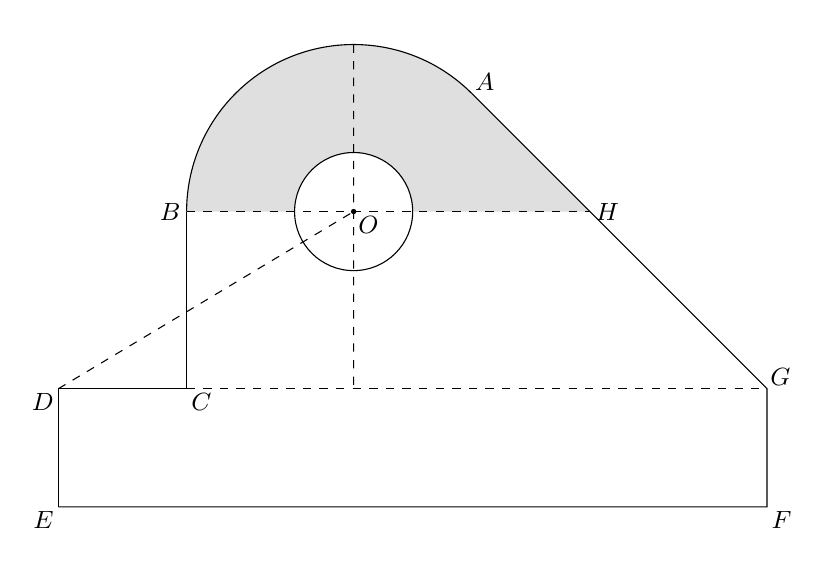
\begin{tikzpicture}[scale=0.75, font=\small]
  \coordinate (D) at (0,2);
  \coordinate (E) at (0,0);
  \coordinate (F) at (12,0);
  \coordinate (G) at (12,2);
  \coordinate (O) at (5,5);
  \coordinate (A) at (7,7);
  \coordinate (B) at (2.1716,5);
  \coordinate (C) at (2.1716,2);
  \coordinate (H) at (9,5);
  \coordinate (T) at (5,7.8284);
  % ---------- 阴影：弧 B→A + AH + HB，随后把圆孔填白 ----------
  \fill[gray!25] (B) arc[start angle=180, end angle=45, radius=2.8284] -- (H) -- cycle;
  \fill[white] (O) circle (1);
  % ---------- 虚线 ----------
  \draw[dashed] (B) -- (H);
  \draw[dashed] (C) -- (G);
  \draw[dashed] (T) -- (5,2);
  \draw[dashed] (D) -- (O);
  % ---------- 实线轮廓与圆孔 ----------
  \draw (E) -- (F) -- (G) -- (A);
  \draw (A) arc[start angle=45, end angle=180, radius=2.8284];
  \draw (B) -- (C);
  \draw (C) -- (D) -- (E);
  \draw (O) circle (1);
  \fill (O) circle (1.3pt);
  % ---------- 标签 ----------
  \node[above right, inner sep=1pt] at (A) {$A$};
  \node[left, inner sep=2pt] at (B) {$B$};
  \node[below right, inner sep=1.5pt] at (C) {$C$};
  \node[below left, inner sep=1.5pt] at (D) {$D$};
  \node[below left, inner sep=1.5pt] at (E) {$E$};
  \node[below right, inner sep=1.5pt] at (F) {$F$};
  \node[above right, inner sep=1pt] at (G) {$G$};
  \node[right, inner sep=2pt] at (H) {$H$};
  \node[below right, inner sep=1.5pt] at (O) {$O$};
\end{tikzpicture}
\end{center}
\nopagebreak[4]
\end{question}
\begin{question}
\gkti{16}已知直四棱柱 $ABCD-A_1B_1C_1D_1$ 的棱长均为 $2$，$\angle BAD=60^\circ$。以 $D_1$ 为球心、$\sqrt5$ 为半径的球面与侧面 $BCC_1B_1$ 的交线长为\gkblank{}。

\end{question}
\gkpart{四、解答题}

\begin{question}
\gkti{17}在 ①$ac=\sqrt3$、②$c\sin A=3$、③$c=\sqrt3b$ 这三个条件中任选一个，补充在下面问题中，若问题中的三角形存在，求 $c$ 的值；若问题中的三角形不存在，说明理由。

问题：是否存在 $\triangle ABC$，它的内角 $A$，$B$，$C$ 的对边分别为 $a$，$b$，$c$，且 $\sin A=\sqrt3\sin B$，$C=\dfrac\pi6$，\gkblank{}？

\end{question}
\begin{question}
\gkti{18}已知公比大于 $1$ 的等比数列 $\{a_n\}$ 满足 $a_2+a_4=20$，$a_3=8$。

（1） 求 $\{a_n\}$ 的通项公式；

（2） 记 $b_m$ 为 $\{a_n\}$ 在区间 $(0,m]$（$m\in\mathbf N^*$）中的项的个数，求数列 $\{b_m\}$ 的前 $100$ 项和 $S_{100}$。

\end{question}
\begin{question}
\gkti{19}为加强环境保护，治理空气污染，环境监测部门对某市空气质量进行调研，随机抽查了 $100$ 天空气中的 PM2.5 和 $\mathrm{SO_2}$ 浓度（单位：$\mu\mathrm g/\mathrm m^3$），得下表：

\begin{center}
\begin{tabular}{cccc}
\toprule
$\mathrm{SO_2}$ 浓度 & $[0,50]$ & $(50,150]$ & $(150,475]$ \\
\midrule
PM2.5 $[0,35]$ & $32$ & $18$ & $4$ \\
PM2.5 $(35,75]$ & $6$ & $8$ & $12$ \\
PM2.5 $(75,115]$ & $3$ & $7$ & $10$ \\
\bottomrule
\end{tabular}
\end{center}

（1） 估计事件「该市一天空气中 PM2.5 浓度不超过 $75$，且 $\mathrm{SO_2}$ 浓度不超过 $150$」的概率；

（2） 根据所给数据，完成下面的 $2\times2$ 列联表：

\begin{center}
\begin{tabular}{ccc}
\toprule
$\mathrm{SO_2}$ 浓度 & $[0,150]$ & $(150,475]$ \\
\midrule
PM2.5 $[0,75]$ &  &  \\
PM2.5 $(75,115]$ &  &  \\
\bottomrule
\end{tabular}
\end{center}

（3） 根据（2）中的列联表，判断是否有 $99\%$ 的把握认为该市一天空气中 PM2.5 浓度与 $\mathrm{SO_2}$ 浓度有关？

\Needspace{10\baselineskip}
附：$K^2=\dfrac{n(ad-bc)^2}{(a+b)(c+d)(a+c)(b+d)}$，

\begin{center}
\begin{tabular}{cccc}
\toprule
$P(K^2\geqslant k)$ & $0.050$ & $0.010$ & $0.001$ \\
\midrule
$k$ & $3.841$ & $6.635$ & $10.828$ \\
\bottomrule
\end{tabular}
\end{center}

\Needspace{0.4\textheight}
\end{question}
\begin{question}
\gkti{20}如图，四棱锥 $P-ABCD$ 的底面为正方形，$PD\perp$ 底面 $ABCD$。设平面 $PAD$ 与平面 $PBC$ 的交线为 $l$。
\nopagebreak[4]
\begin{center}% 2020 新高考Ⅰ卷（山东）20：四棱锥 P-ABCD（底面 ABCD 为正方形，PD⊥底面 ABCD）
% 绘制依据：固定源 PDF 原页。底面按斜二测画：A 左前、B 右前、C 右后、D 中后（被遮挡顶点）；
% PD 垂直底面，故 P 画在 D 的正上方（位于版面中偏左）。
% 实线：PA、PB、PC、AB、BC；虚线：PD、AD、DC。只标 P、A、B、C、D 五点。
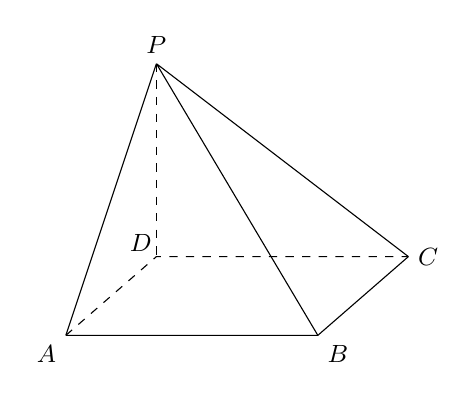
\begin{tikzpicture}[scale=1.0, font=\small]
  \coordinate (A) at (0,0);
  \coordinate (B) at (3.2,0);
  \coordinate (C) at (4.35,1.0);
  \coordinate (D) at (1.15,1.0);
  \coordinate (P) at (1.15,3.45);
  \draw (P) -- (A)  (P) -- (B)  (P) -- (C);
  \draw (A) -- (B) -- (C);
  \draw[dashed] (P) -- (D);
  \draw[dashed] (A) -- (D) -- (C);
  \node[above] at (P) {$P$};
  \node[below left] at (A) {$A$};
  \node[below right] at (B) {$B$};
  \node[right] at (C) {$C$};
  \node[above left, inner sep=1.5pt] at (D) {$D$};
\end{tikzpicture}
\end{center}
\nopagebreak[4]
（1） 证明：$l\perp$ 平面 $PDC$；

（2） 已知 $PD=AD=1$，$Q$ 为 $l$ 上的点，求 $PB$ 与平面 $QCD$ 所成角的正弦值的最大值。

\end{question}
\begin{question}
\gkti{21}已知函数 $f(x)=a\mathrm e^{x-1}-\ln x+\ln a$。

（1） 当 $a=\mathrm e$ 时，求曲线 $y=f(x)$ 在点 $(1,f(1))$ 处的切线与两坐标轴围成的三角形的面积；

（2） 若 $f(x)\geqslant1$，求 $a$ 的取值范围。

\end{question}
\begin{question}
\gkti{22}已知椭圆 $C:\dfrac{x^2}{a^2}+\dfrac{y^2}{b^2}=1$（$a>b>0$）的离心率为 $\dfrac{\sqrt2}2$，且过点 $A(2,1)$。

（1） 求 $C$ 的方程；

（2） 点 $M$，$N$ 在 $C$ 上，且 $AM\perp AN$，$AD\perp MN$，$D$ 为垂足。证明：存在定点 $Q$，使得 $|DQ|$ 为定值。

\end{question}